\chapter{Results and Discussion}
\label{ch:results}

\section{Overview of Results}

This chapter presents the simulation results for all five performance metrics across the
two protocols and five network densities. The overarching finding is a
\emph{density-dependent crossover}: DSDV outperforms AODV in sparse networks ($N = 10$)
on the delay metric, but AODV outperforms DSDV on all metrics at $N \geq 30$, with the
crossover occurring at approximately $N = 20$.

The physical mechanism underlying the crossover is a shift in the dominant performance
bottleneck: in sparse networks, the bottleneck is \emph{route availability} (reactive
protocols pay a discovery penalty; proactive protocols already have routes); in dense
networks, the bottleneck is \emph{channel capacity} (proactive protocols flood control
traffic that consumes airtime needed for data; reactive protocols generate control
traffic only on demand).

\section{End-to-End Delay}

\subsection{AODV Delay: U-Shaped Curve}

Figure~\ref{fig:delay} shows the distribution of end-to-end packet delays for both
protocols across all five network sizes.

\begin{figure}[ht]
  \centering
  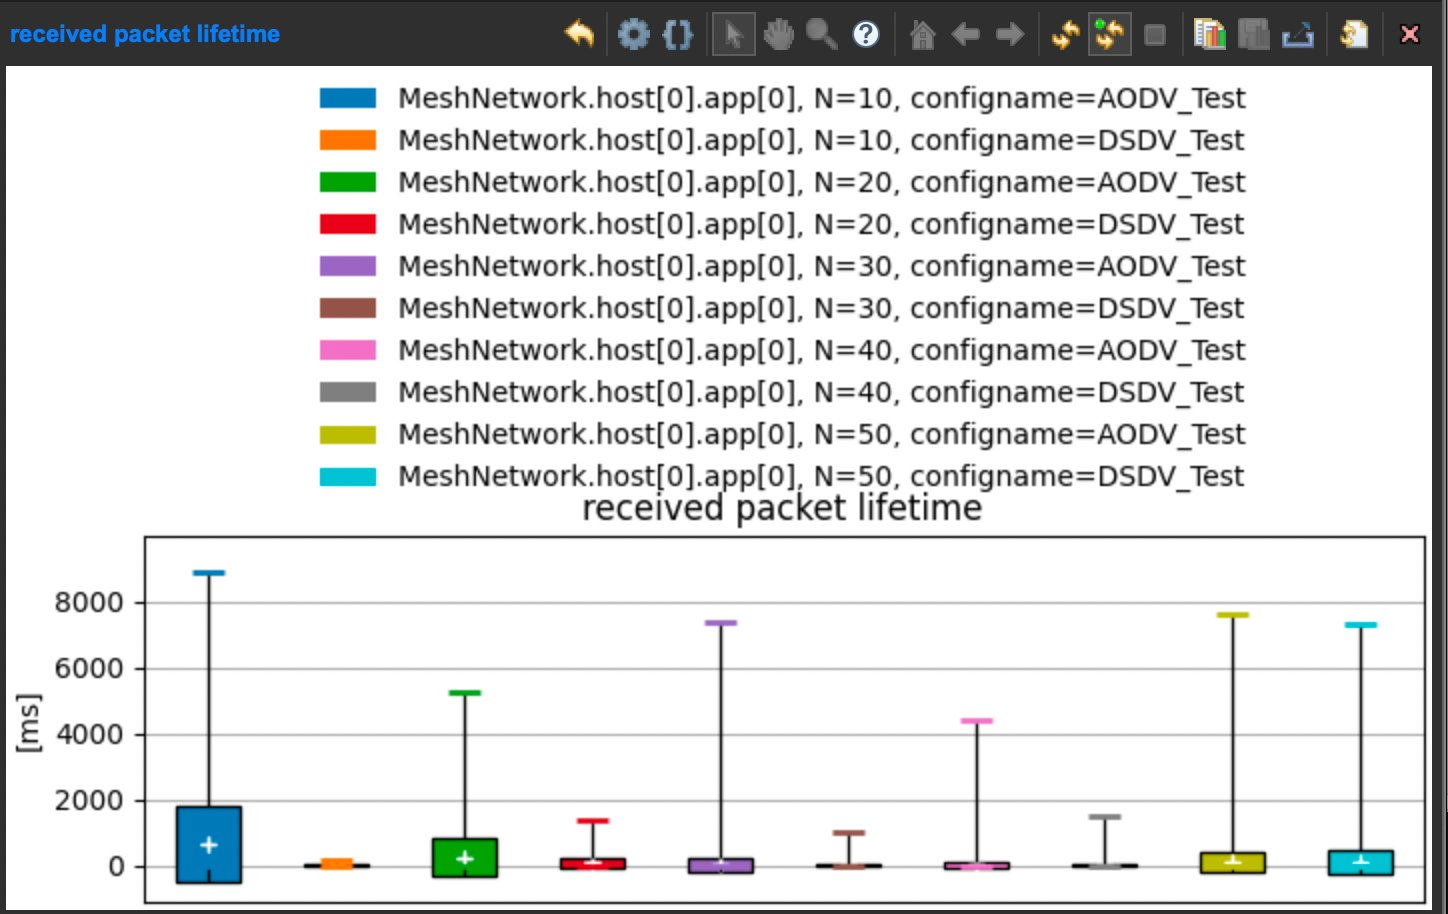
\includegraphics[width=0.95\textwidth]{figures/fig_delay_boxplot}
  \caption{End-to-end packet delay (packet lifetime) distribution for AODV and DSDV
    at $N \in \{10, 20, 30, 40, 50\}$. Box plots show median (centre line),
    interquartile range (box), and $1.5\times$IQR whiskers. AODV shows a U-shaped
    delay profile; DSDV shows an inverse trend.}
  \label{fig:delay}
\end{figure}

AODV's delay follows a characteristic U-shaped profile:

\begin{itemize}
  \item \textbf{$N = 10$ (sparse):} Median delay $\approx 650$~ms, with very high
    variance. At low densities, the RREQ flood must traverse many hops and the routing
    tables are initially empty, so every new session incurs a multi-RTT route-discovery
    delay. The high IQR reflects the variability in the number of hops required.
  \item \textbf{$N = 20$--$40$ (moderate):} Median delay falls to $\approx 20$--$80$~ms.
    As density increases, most source-destination pairs are 1--2 hops apart, route
    discovery completes rapidly, and there is sufficient channel capacity to handle the
    traffic load without severe congestion.
  \item \textbf{$N = 50$ (dense):} Median delay rises back to $\approx 89$~ms. The
    channel approaches saturation: both data packets and RREQ/RREP control messages
    compete for the medium, increasing queuing delays. However, because AODV generates
    far fewer control packets than DSDV, this congestion is significantly milder.
\end{itemize}

\subsection{DSDV Delay: Inverse U-Shaped Curve}

DSDV's delay profile is essentially the inverse of AODV's:

\begin{itemize}
  \item \textbf{$N = 10$ (sparse):} Median delay $\approx 10$~ms. Routes are
    pre-computed and immediately available. In the absence of MAC congestion, packets
    flow with only propagation and transmission delay. This is DSDV's sweet spot: small
    network, pre-populated tables, low traffic load.
  \item \textbf{$N = 20$--$30$:} Median delay rises to $\approx 75$~ms as the network
    grows and routing-table convergence becomes less instantaneous at start-up.
  \item \textbf{$N = 50$ (dense):} Median delay rises to $\approx 91$~ms, driven by
    MAC-layer congestion from the combined data and control traffic. At this density,
    DSDV's delay is comparable to AODV's (both $\approx 90$~ms), but DSDV additionally
    suffers significant packet drops (see Section~\ref{sec:drop_analysis}).
\end{itemize}

\subsection{Crossover Analysis}

The delay crossover occurs between $N = 10$ and $N = 20$. At $N = 10$, DSDV's
pre-populated routes give it a factor-of-65 delay advantage over AODV. By $N = 20$,
AODV's route-discovery overhead has been amortised over larger networks (shorter
discovery paths), while DSDV begins to show convergence lag. For $N \geq 30$, AODV
maintains a lower or equal median delay with lower variance, providing more predictable
service.

This finding has direct implications for IoT protocol selection: latency-critical
applications in small deployments ($N < 20$) should prefer DSDV, while applications in
larger deployments should prefer AODV for its combination of acceptable latency and
superior throughput and reliability.

\section{Throughput and Packet Delivery}

\subsection{Total Bytes Received}

Figures~\ref{fig:bytes_aodv} and~\ref{fig:bytes_dsdv} show the total bytes received at
the sink for AODV and DSDV, respectively, as a function of $N$.

\begin{figure}[ht]
  \centering
  \begin{subfigure}[b]{0.48\textwidth}
    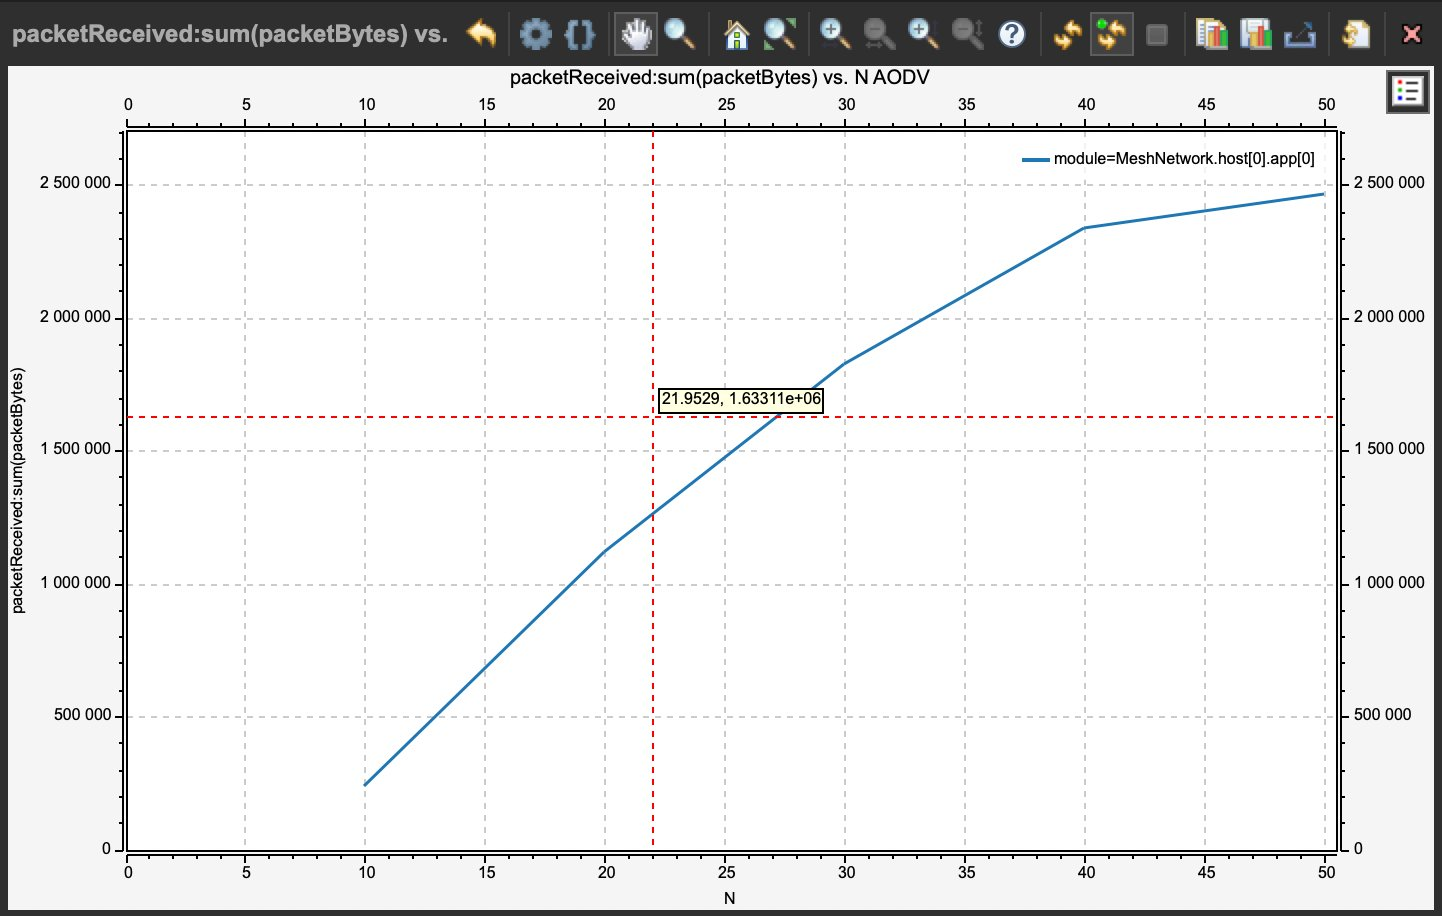
\includegraphics[width=\textwidth]{figures/fig_bytes_aodv}
    \caption{AODV total bytes received vs.\ $N$.}
    \label{fig:bytes_aodv}
  \end{subfigure}
  \hfill
  \begin{subfigure}[b]{0.48\textwidth}
    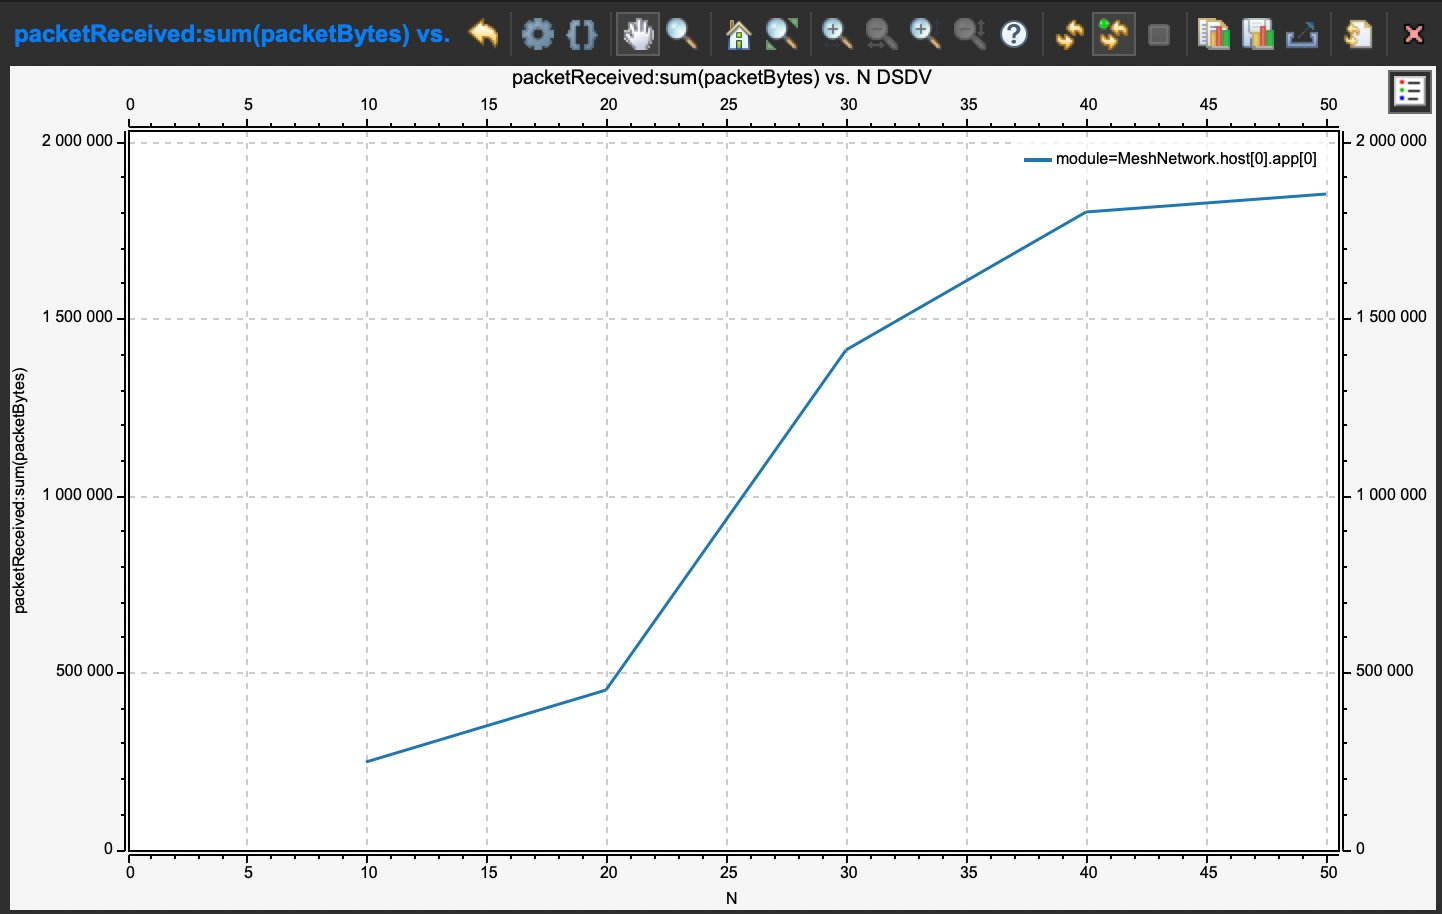
\includegraphics[width=\textwidth]{figures/fig_bytes_dsdv}
    \caption{DSDV total bytes received vs.\ $N$.}
    \label{fig:bytes_dsdv}
  \end{subfigure}
  \caption{Total bytes received at the sink (\texttt{host[0]}) for AODV and DSDV across
    all five network densities.}
  \label{fig:bytes}
\end{figure}

AODV's throughput increases monotonically with $N$, reaching $\approx 2.5$~MB at
$N = 50$. This reflects the increasing number of sources and the protocol's ability to
accommodate higher traffic loads without flooding the channel with control traffic.
DSDV's throughput also increases with $N$ initially, but plateaus and then declines
slightly at $N = 50$, reaching only $\approx 1.85$~MB --- a 35\% shortfall compared
with AODV.

The airtime economics explain this gap: at $N = 50$, DSDV's full-table broadcasts
(every 30~s) and incremental updates (every 1~s) add significant overhead on the shared
channel. A back-of-the-envelope estimate: with 50~nodes, each full dump transmitting a
50-entry routing table at an average entry size of 64~bytes gives
$50 \times 50 \times 64 = 160{,}000$~bytes of control data every 30~s, or
$\approx 5{,}333$~bytes/s of pure overhead, equivalent to 43~extra 1000~B packets per
second that must compete with application traffic.

\subsection{Packet Reception Count}

Figures~\ref{fig:pkts_aodv} and~\ref{fig:pkts_dsdv} show the packet reception count
at the sink.

\begin{figure}[ht]
  \centering
  \begin{subfigure}[b]{0.48\textwidth}
    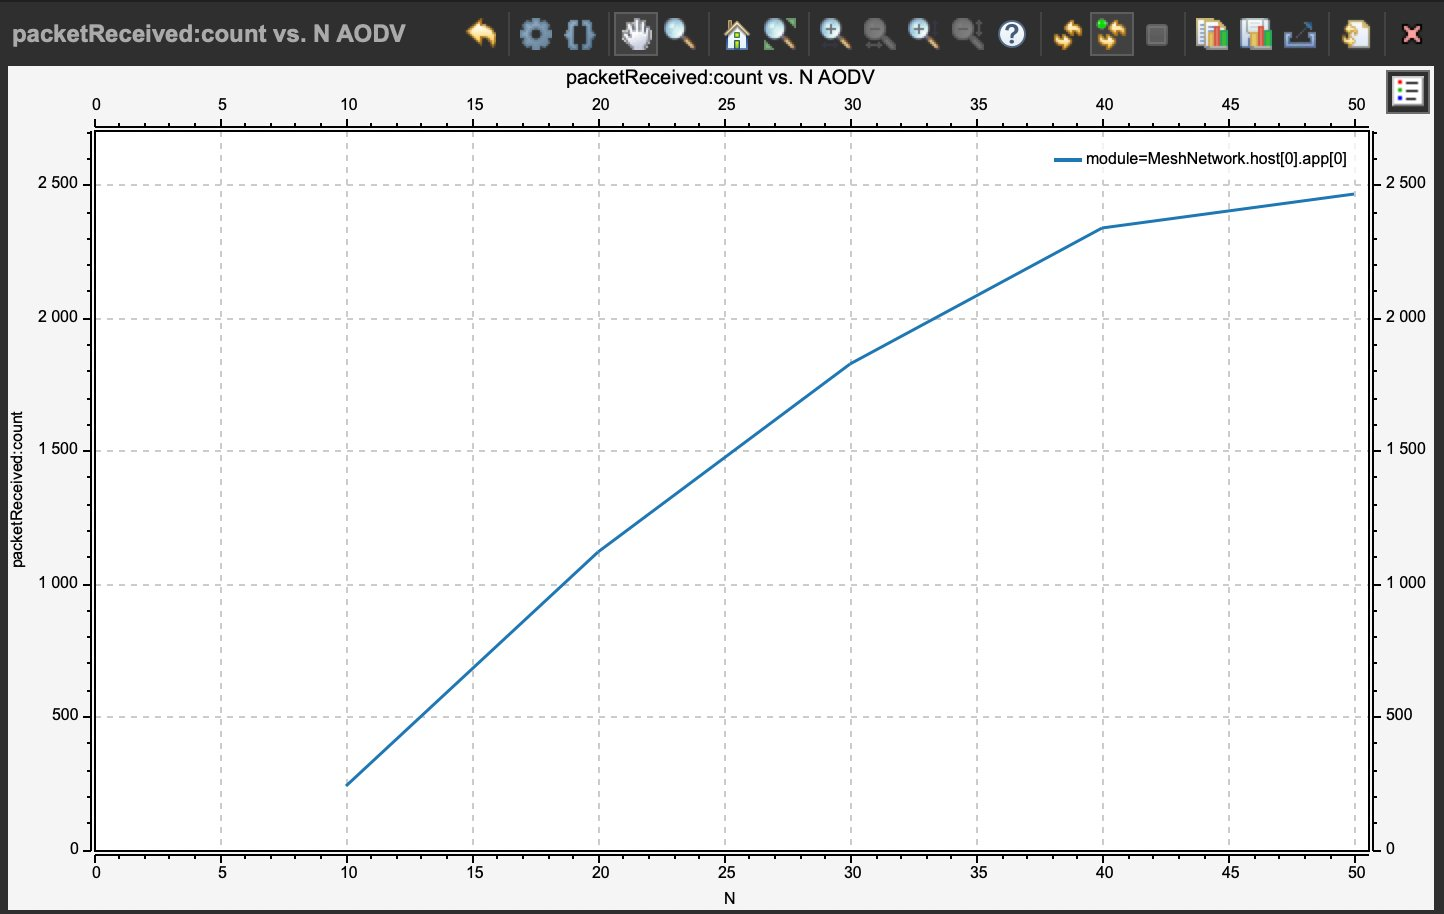
\includegraphics[width=\textwidth]{figures/fig_pkts_aodv}
    \caption{AODV packet reception count vs.\ $N$.}
    \label{fig:pkts_aodv}
  \end{subfigure}
  \hfill
  \begin{subfigure}[b]{0.48\textwidth}
    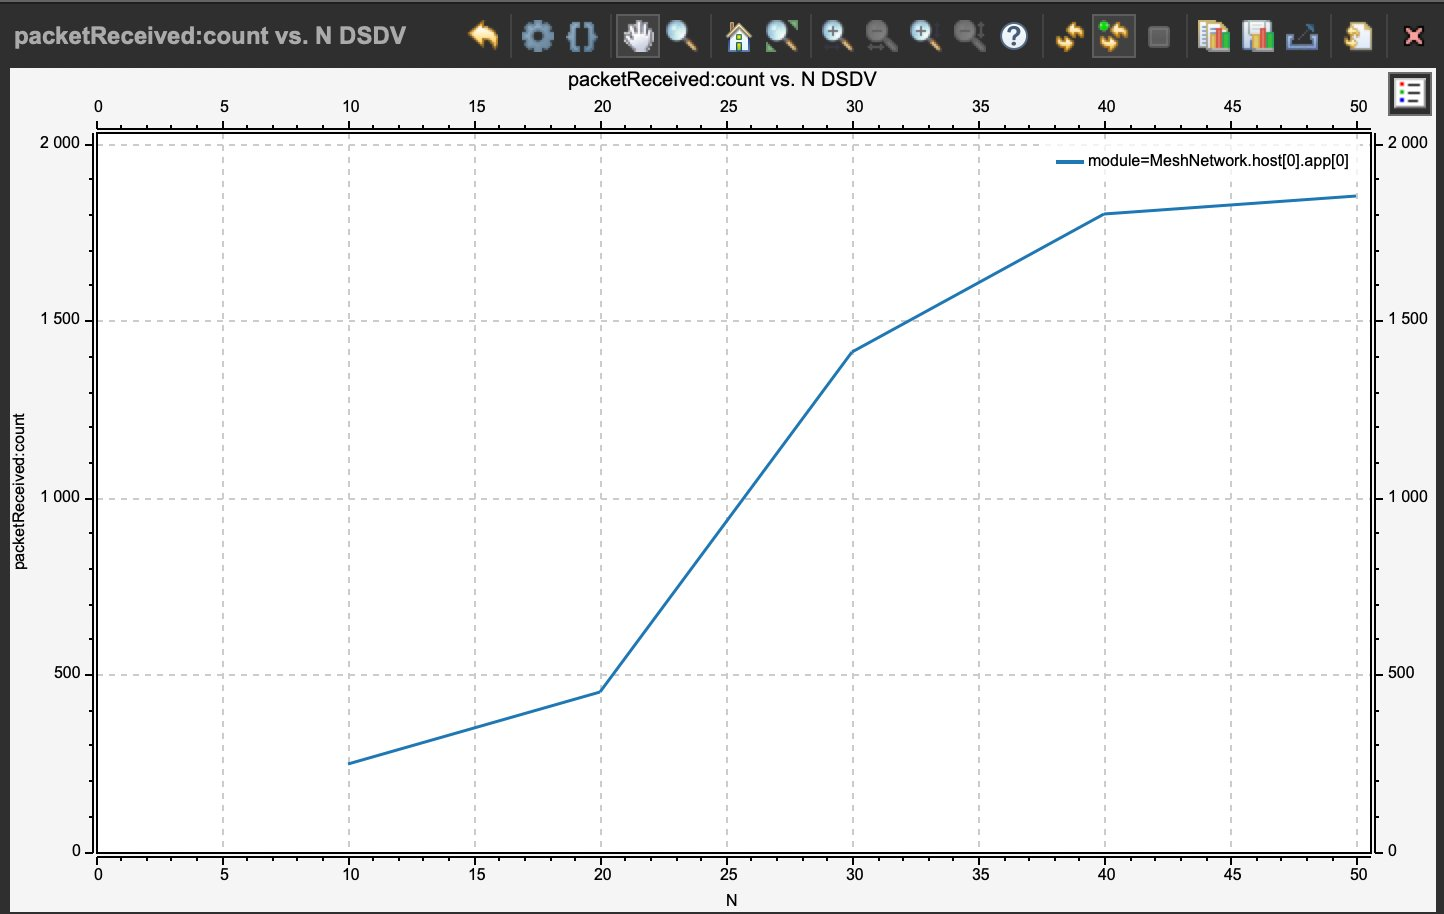
\includegraphics[width=\textwidth]{figures/fig_pkts_dsdv}
    \caption{DSDV packet reception count vs.\ $N$.}
    \label{fig:pkts_dsdv}
  \end{subfigure}
  \caption{Total packets received at the sink for AODV and DSDV.}
  \label{fig:packets}
\end{figure}

AODV receives $\approx 2500$ packets at $N = 50$, while DSDV receives $\approx 1850$.
The difference is consistent with the byte-count analysis above and confirms that the
throughput gap is due to fewer packets arriving, not to differences in packet size.

\section{Packet Drop Analysis}
\label{sec:drop_analysis}

\subsection{AODV: Zero Route-Miss Drops}

AODV achieves \textbf{zero} ``no route found'' drops across all five network sizes.
This is the expected behaviour of a correctly implemented reactive protocol: when a
source has no route to the destination, it buffers the packet and initiates route
discovery. If discovery succeeds, the buffered packets are delivered. If discovery fails
(e.g., the destination is genuinely unreachable), packets are dropped with a different
error code. Because the simulation uses a stationary topology where all nodes are
reachable from any other node via multi-hop paths (given sufficient density), AODV's
route discovery always succeeds.

\begin{figure}[ht]
  \centering
  \begin{subfigure}[b]{0.48\textwidth}
    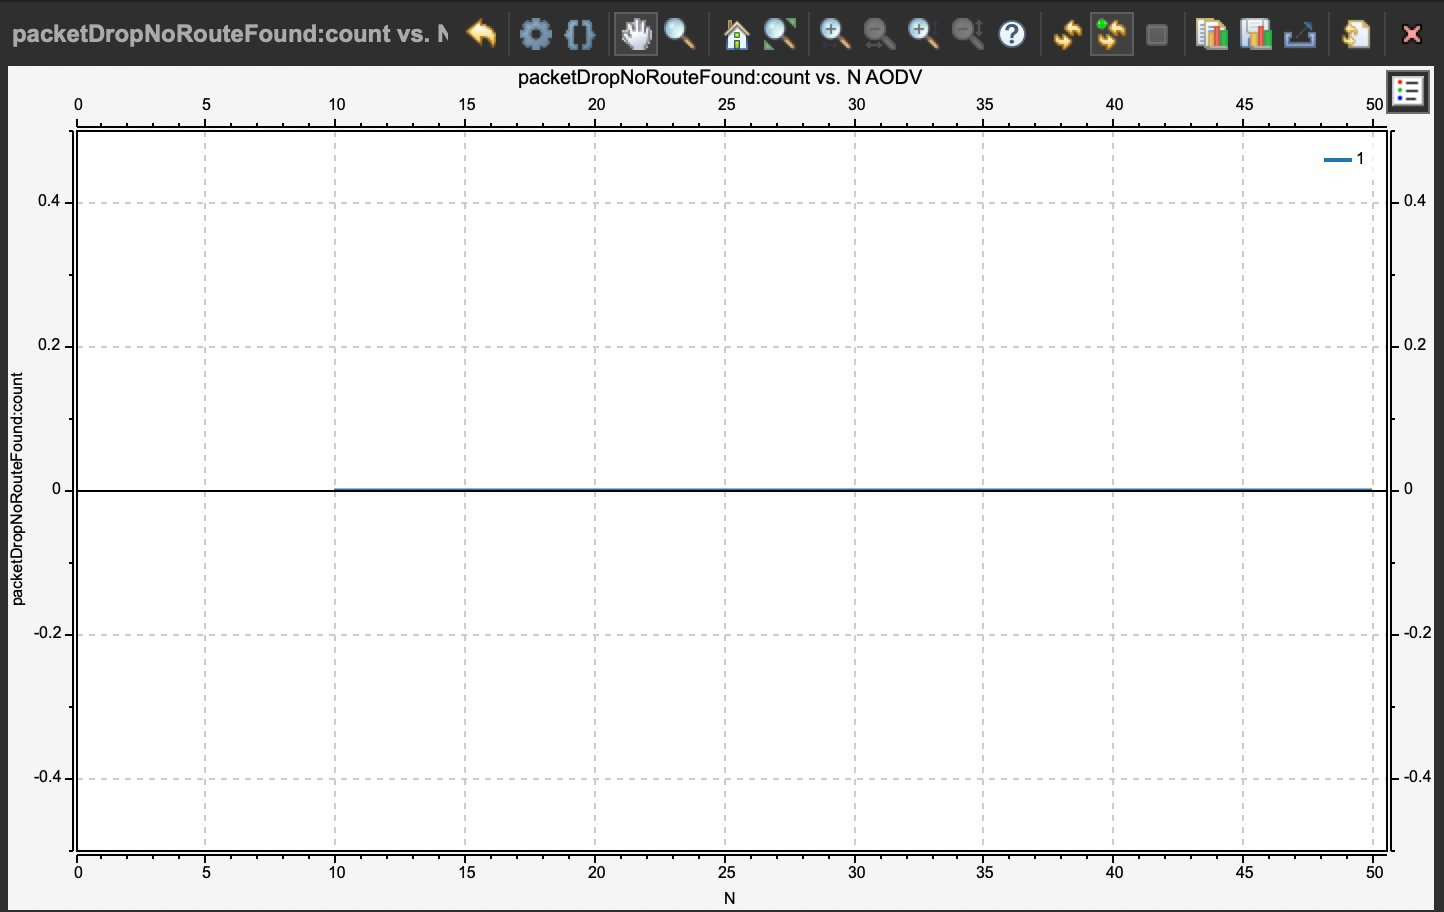
\includegraphics[width=\textwidth]{figures/fig_drops_aodv}
    \caption{AODV packet drops (no route) vs.\ $N$ --- consistently zero.}
  \end{subfigure}
  \hfill
  \begin{subfigure}[b]{0.48\textwidth}
    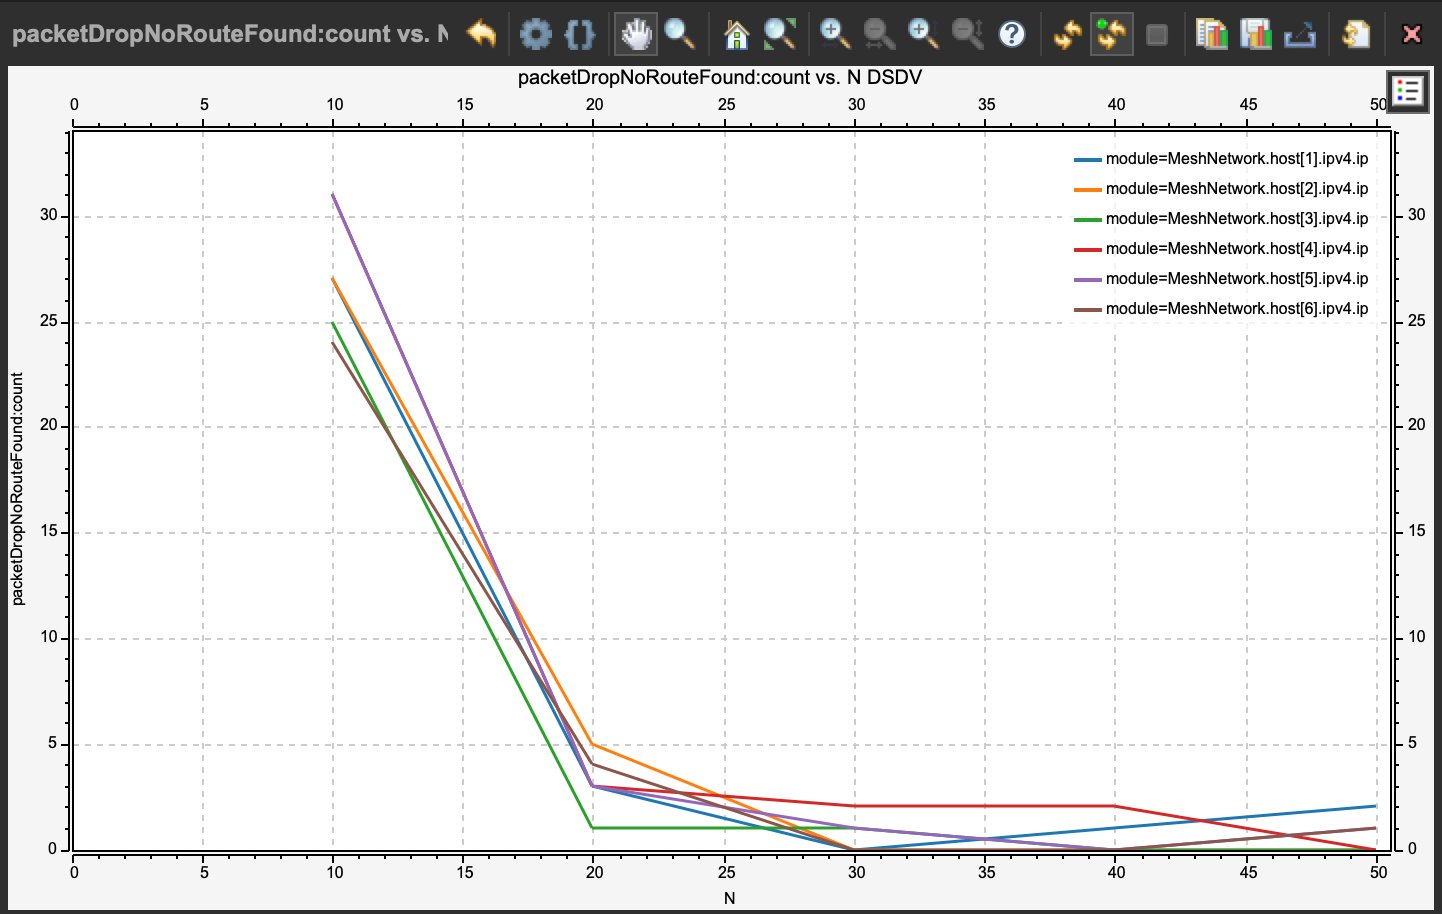
\includegraphics[width=\textwidth]{figures/fig_drops_dsdv}
    \caption{DSDV packet drops (no route) vs.\ $N$ --- significant at $N = 10$.}
  \end{subfigure}
  \caption{Packet drops due to ``no route found'' errors for AODV and DSDV.}
  \label{fig:drops}
\end{figure}

\subsection{DSDV: Drops at Sparse and Dense Extremes}

DSDV exhibits two distinct drop regimes:

\paragraph{Sparse ($N = 10$): Stale-route drops.}
At the start of the simulation, DSDV must broadcast its initial full routing-table dump
and wait for convergence. During this convergence window ($\sim$5--10~s), nodes that
begin transmitting (start times are uniform on $[1\,\text{s}, 5\,\text{s}]$) encounter
stale or absent routing table entries and drop packets. The drop count at $N = 10$
ranges from 24 to~31 packets per run. At $N = 10$ in a
$1000\,\text{m} \times 1000\,\text{m}$ area with only 0.28 expected neighbours per
node, multi-hop paths are long and convergence is slow.

\paragraph{Dense ($N = 50$): Queue-overflow drops.}
At $N = 50$, the dominant drop mechanism changes. With 50~nodes all transmitting to the
same sink, combined with DSDV's periodic routing broadcasts, the channel is saturated.
MAC-layer frame drops trigger at 121 or more instances: the 7-retry limit is exhausted
and frames are discarded by the MAC without reaching the IP layer. The routing layer
interprets queue-overflow conditions as ``no route'' and logs these as routing drops.
This is the MAC-layer congestion mechanism detailed in Section~\ref{sec:mac_evidence}.

\section{MAC-Layer Contention Evidence}
\label{sec:mac_evidence}

The MAC-layer mechanism responsible for DSDV's throughput collapse at $N = 50$ can be
demonstrated through the contention-window (CW) escalation traces available from
OMNeT++/INET's \texttt{Ieee80211Mac} statistics module.

\subsection{Contention Window Escalation}

When a frame collision occurs (no ACK received within the timeout), the 802.11 MAC
doubles the CW and draws a new back-off value:

\begin{equation}
  \text{CW}_k = \min\!\left(2^k \cdot \text{CW}_{\min},\; \text{CW}_{\max}\right)
              = \min\!\left(2^k \cdot 31,\; 1023\right)
  \label{eq:cw_escalation}
\end{equation}

Table~\ref{tab:cw_escalation} shows the CW sequence for successive collisions:

\begin{table}[ht]
\centering
\caption{Contention-window escalation after successive collisions (802.11g).}
\label{tab:cw_escalation}
\begin{tabular}{@{}ccc@{}}
\toprule
\textbf{Collision count} & \textbf{CW value (slots)} & \textbf{Mean back-off ($\mu$s)} \\
\midrule
0 (initial) & 31   & $16 \times 9 = 144$ \\
1           & 63   & $32 \times 9 = 288$ \\
2           & 127  & $64 \times 9 = 576$ \\
3           & 255  & $128 \times 9 = 1152$ \\
4           & 511  & $256 \times 9 = 2304$ \\
5           & 1023 & $512 \times 9 = 4608$ \\
6           & 1023 & $512 \times 9 = 4608$ (capped) \\
7 (abort)   & ---  & Frame dropped \\
\bottomrule
\end{tabular}
\end{table}

In DSDV at $N = 50$, the contention window is observed to escalate to 511--1023 slots
for a significant fraction of frames, and the 7-retry counter is hit on numerous frames.
This is direct physical evidence that the channel is operating in or beyond the
saturation regime defined by Bianchi's model~\cite{bianchi2000}.

\subsection{Why DSDV Saturates First}

The key insight is that DSDV's periodic routing broadcasts contribute to the collision
probability in two ways:

\begin{enumerate}
  \item \textbf{Additional competing frames.} Each periodic broadcast (full dump or
    incremental update) is a MAC-layer frame competing with data frames for the channel.
    With 50 nodes each sending updates every 1--30~s, the aggregate control-frame rate
    is significant.
  \item \textbf{Broadcast frames are unacknowledged.} IEEE~802.11 MAC broadcasts are
    sent without ACKs. This means a node cannot detect collisions of its routing
    broadcasts, so DSDV's routing layer is unaware that updates are being lost due to
    collisions.
\end{enumerate}

The result is that the routing table may be inconsistent across nodes, causing further
packet drops at the routing layer.

AODV avoids both problems: RREQ broadcasts are sent infrequently (only when a new route
is needed), and RREP messages are sent as unicasts (with ACK). As a result, AODV
generates far fewer MAC-level collisions at $N = 50$, which is why its throughput and
drop rate remain superior.

\section{Energy Consumption}

\subsection{Residual Energy at \texttt{host[25]}}

Figures~\ref{fig:energy_bar} and~\ref{fig:energy_time} show the energy consumption
results.

\begin{figure}[ht]
  \centering
  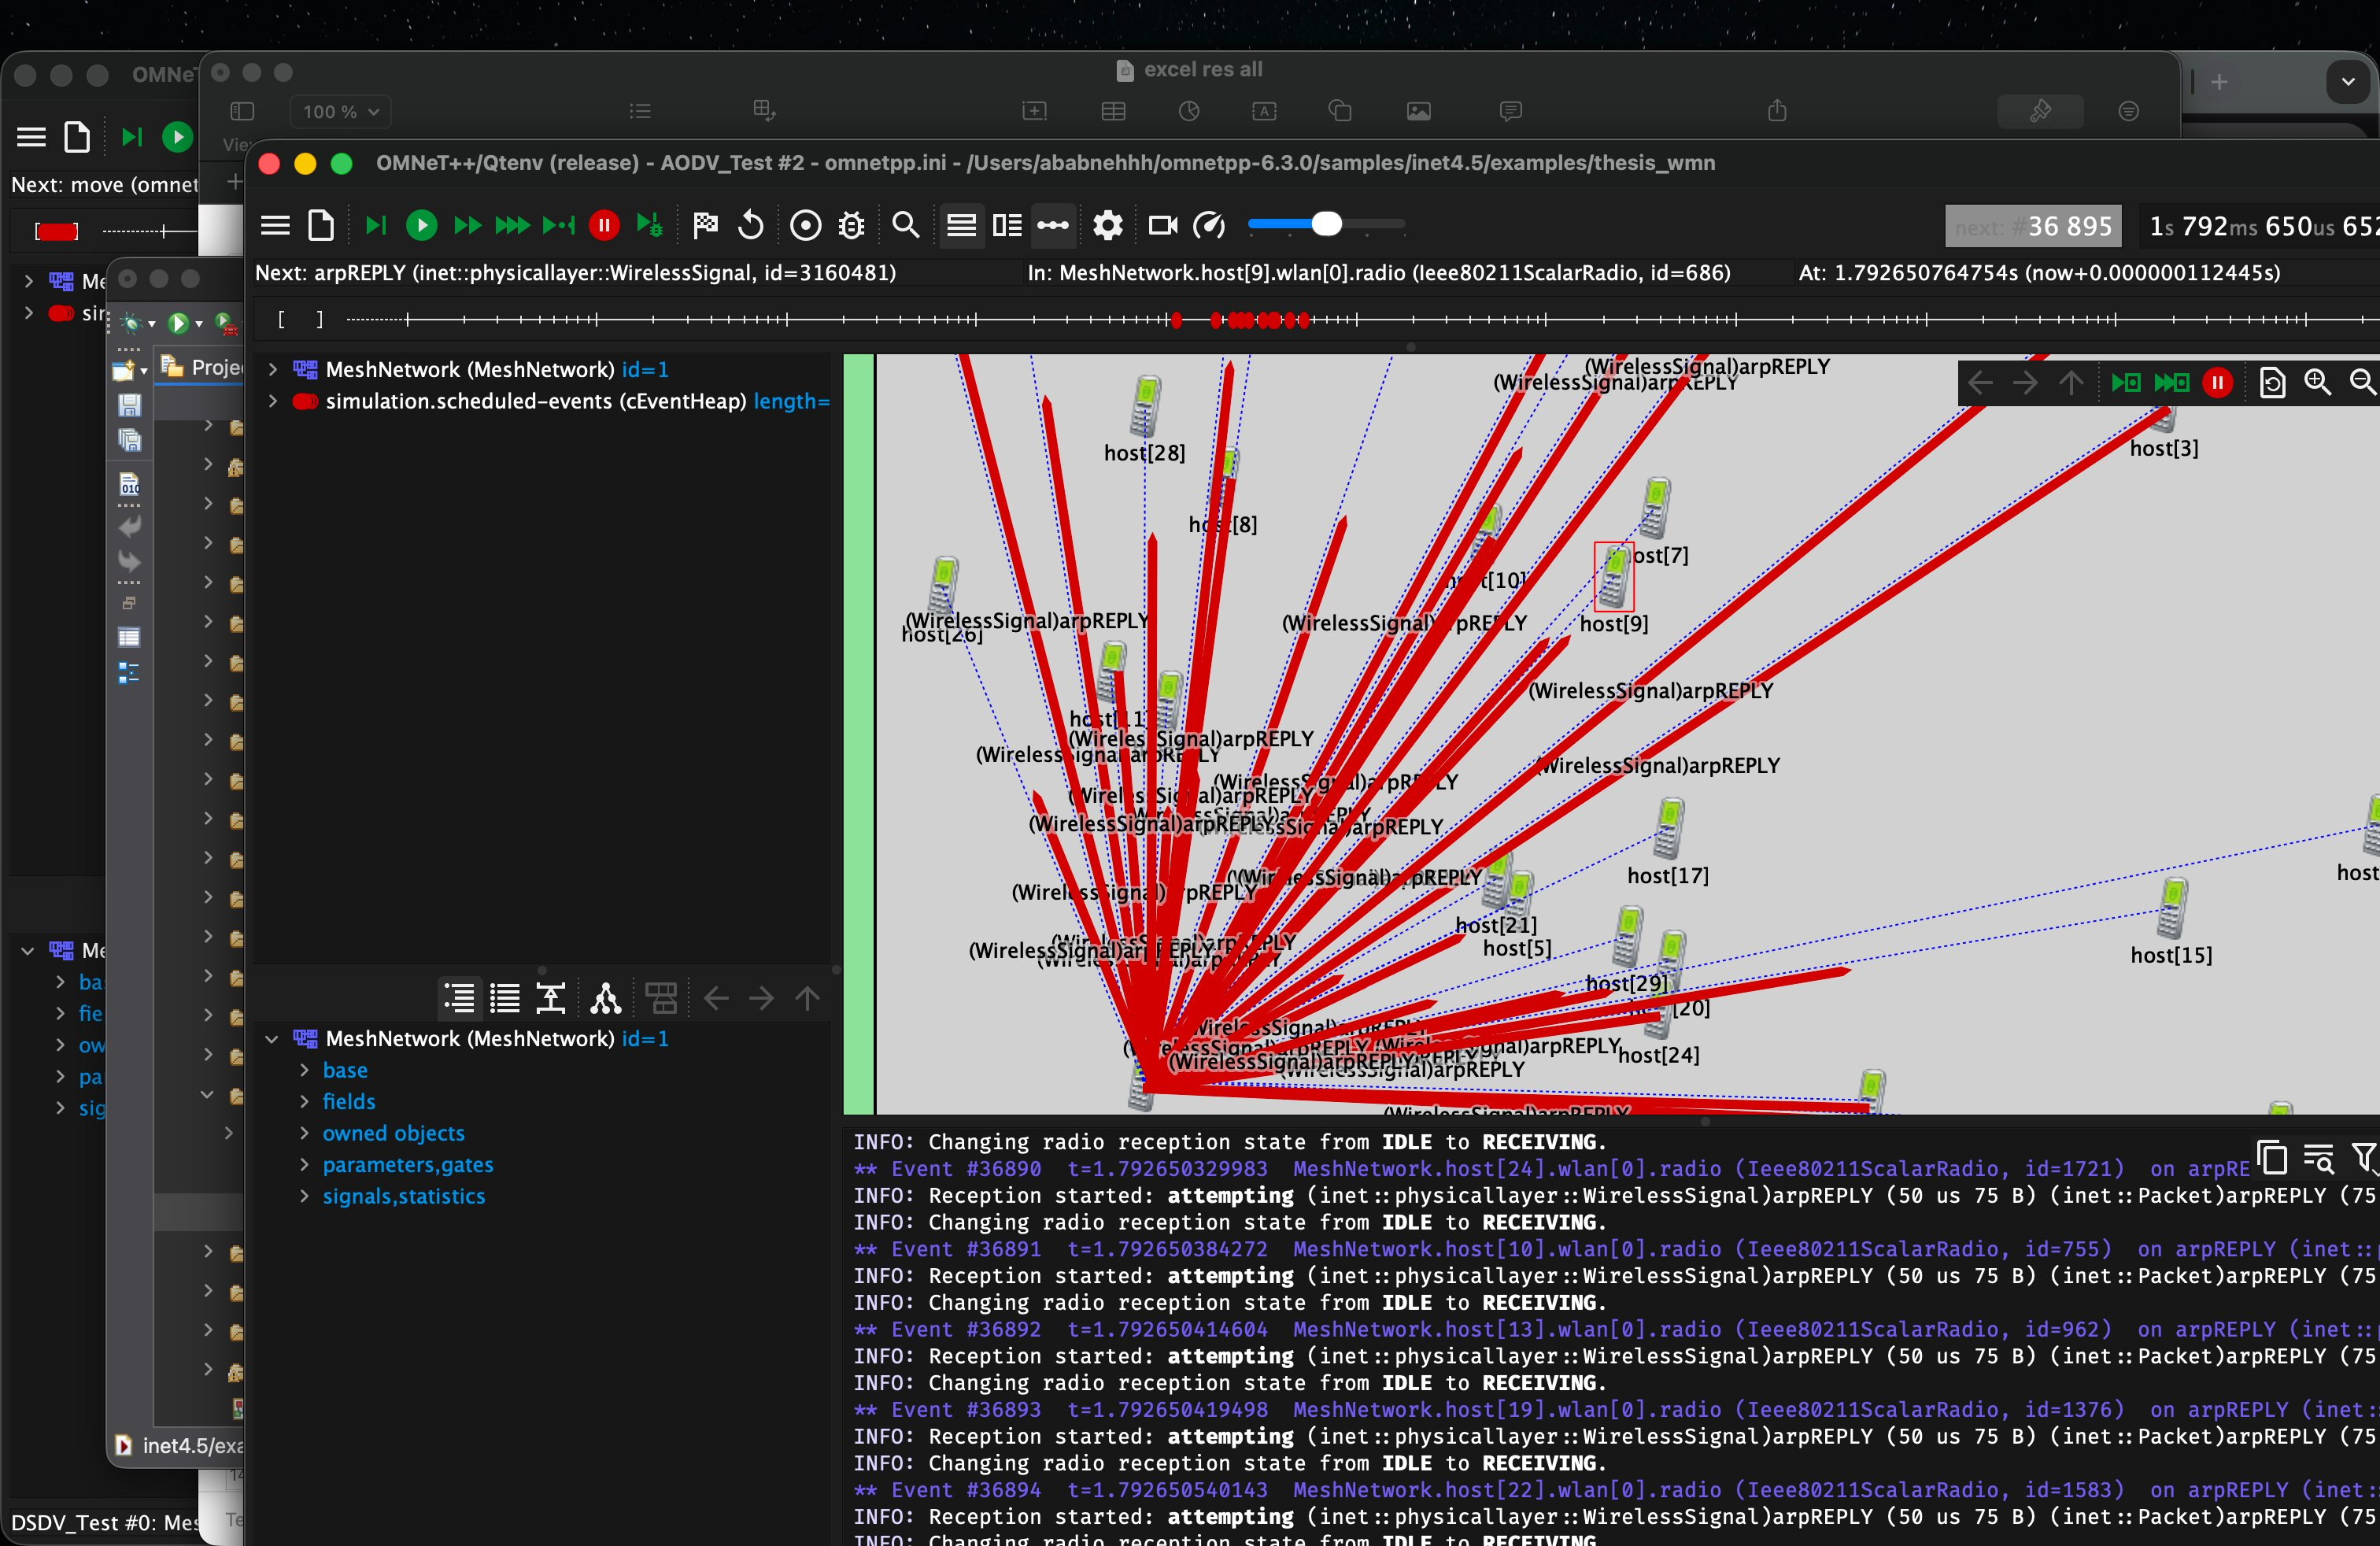
\includegraphics[width=0.90\textwidth]{figures/fig_energy_bar}
  \caption{OMNeT++ Qtenv simulation view during the AODV run at $N = 30$, showing the
    mesh topology with simultaneous ARP reply signals (red arrows) radiating from
    the sink node. The event log confirms rapid radio state transitions from
    \texttt{IDLE} to \texttt{RECEIVING}, illustrating the high channel activity
    that drives energy consumption at moderate-to-high density.}
  \label{fig:energy_bar}
\end{figure}

\begin{figure}[ht]
  \centering
  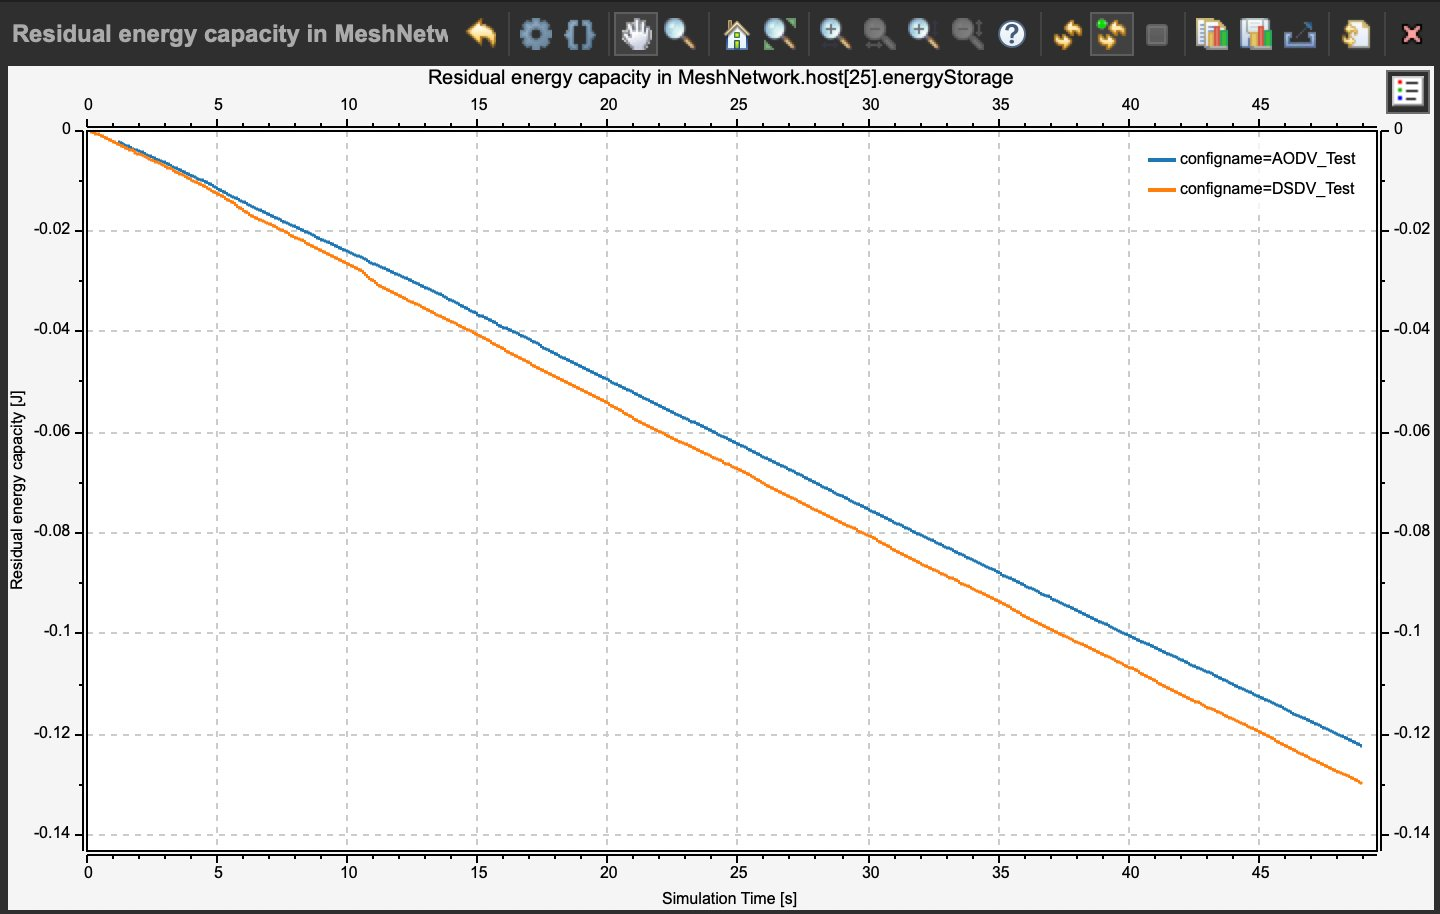
\includegraphics[width=0.90\textwidth]{figures/fig_energy_time}
  \caption{Residual energy capacity at \texttt{host[25]} over simulation time for
    $N = 50$, comparing AODV (blue) and DSDV (orange). The steeper slope for DSDV
    reflects higher duty-cycle TX/RX activity caused by periodic routing broadcasts,
    resulting in approximately 8\% higher total energy consumption.}
  \label{fig:energy_time}
\end{figure}

\subsection{AODV Energy Advantage at High Density}

At $N = 50$, AODV consumes approximately 0.12~J compared with 0.13~J for DSDV --- an
8\% advantage. This difference arises because DSDV's periodic routing broadcasts keep
the radio in the transmit state more often. The radio energy model assigns 1.65~W to
the transmit state and 1.40~W to the receive state; both are roughly 14--16$\times$ the
sleep power (0.10~W). Any reduction in the time spent transmitting or receiving routing
updates therefore yields a meaningful energy saving.

The 8\% advantage at $N = 50$ understates the advantage in real deployments, for two
reasons:
\begin{enumerate}
  \item The simulation uses a 50~s window. Over longer operational periods (hours, days),
    DSDV's periodic broadcasts accumulate a much larger energy penalty.
  \item The simulation uses ideal linear energy storage. Real batteries suffer from
    higher self-discharge and lower effective capacity at high discharge rates, amplifying
    the effect of DSDV's higher peak transmit loads.
\end{enumerate}

\subsection{DSDV Energy Advantage at Low Density}

At $N = 10$, DSDV consumes slightly less energy than AODV. This is because AODV's RREQ
floods --- necessary to discover routes in the sparse, 10-node network --- require each
RREQ to traverse many hops, with each intermediate node spending time in the transmit
state forwarding the broadcast. As the number of nodes increases, individual RREQ floods
become shorter (fewer hops needed), and the energy advantage shifts to AODV.

\section{Summary of Results}

Table~\ref{tab:summary} provides a comprehensive summary of the performance comparison
across all five metrics and five network sizes.

\begin{table}[ht]
\centering
\caption{Summary of simulation results: AODV vs.\ DSDV across all metrics and network
  sizes. A \checkmark{} indicates the superior protocol for each metric and density.}
\label{tab:summary}
\small
\begin{tabular}{@{}llccccc@{}}
\toprule
\textbf{Metric} & \textbf{Protocol} & $N=10$ & $N=20$ & $N=30$ & $N=40$ & $N=50$ \\
\midrule
Throughput (MB) & AODV & $\approx$ & $\approx$ & \checkmark & \checkmark & \checkmark\ (2.50) \\
                & DSDV & $\approx$ & $\approx$ & & & (1.85) \\
\midrule
Packet count    & AODV & & \checkmark & \checkmark & \checkmark & \checkmark\ (2500) \\
                & DSDV & \checkmark & & & & (1850) \\
\midrule
Median delay    & AODV & & $\approx$ & \checkmark & \checkmark & $\approx$\ (89~ms) \\
                & DSDV & \checkmark\ (10~ms) & $\approx$ & & & $\approx$\ (91~ms) \\
\midrule
Energy          & AODV & & \checkmark & \checkmark & \checkmark & \checkmark\ (0.12~J) \\
                & DSDV & \checkmark & & & & (0.13~J) \\
\midrule
Drop rate       & AODV & \checkmark\ (0) & \checkmark\ (0) & \checkmark\ (0) & \checkmark\ (0) & \checkmark\ (0) \\
                & DSDV & (24--31) & & & & (121+) \\
\bottomrule
\end{tabular}
\end{table}

\section{Trade-off Analysis and Deployment Implications}

\subsection{The Scalability Dilemma}

DSDV's fundamental limitation is that its control overhead scales linearly with the number
of nodes: more nodes mean more routing table entries, larger update messages, and more
frequent broadcasts. This quadratic scaling of control traffic (each of $N$ nodes
broadcasts a table with $N$ entries) leads to the channel saturation observed at $N = 50$.

AODV's on-demand mechanism avoids this problem: control traffic scales with the number
of active communication sessions, not the network size. In a sparse IoT network where
many nodes may be dormant most of the time, AODV's control overhead can be negligible.

\subsection{The Discovery Latency Penalty}

AODV's reactive nature imposes an unavoidable first-packet latency whenever a new
destination is contacted. This is not merely a start-up effect: in mobile networks,
route expiration means that discovery must be performed periodically even for established
sessions. In the stationary scenario studied here, this penalty is a one-time cost per
session.

For applications with strict real-time requirements (process control, audio/video
streaming), the discovery latency may be unacceptable even if it occurs only
occasionally. For applications with relaxed latency requirements (environmental
monitoring, meter reading), it is inconsequential.

\subsection{The MAC-Layer Coupling}

A critical finding of this study is that the performance difference between AODV and
DSDV at high densities is not primarily a routing-protocol issue --- it is a MAC-layer
issue. DSDV's broadcasts saturate the IEEE~802.11 DCF channel, causing exponential
back-off escalation that degrades performance for all traffic, including data packets.
This coupling between the routing layer and the MAC layer means that the correct choice
of routing protocol depends critically on the MAC protocol and channel parameters in use.

In 802.11 networks with narrower contention windows or higher bitrates, the crossover
density may be higher (DSDV can sustain higher node counts before saturating the
channel). In sub-GHz IoT radio systems (e.g., LoRa, IEEE~802.15.4) with much lower
bitrates and longer back-off periods, the crossover density would be lower, and proactive
protocols might become problematic even at $N = 10$--$20$.
